\documentclass[12pt]{article}

\usepackage{datetime}

\usepackage[T1]{fontenc}
\usepackage{amsmath, amssymb, amsthm}
\usepackage{enumerate}
\usepackage{verbatim}
\usepackage{listings}
\usepackage{fullpage}
\usepackage{graphicx}
\usepackage[dvipsnames]{xcolor}
\usepackage{hyperref}

\newcommand{\hwno}{1}
\newcommand{\duemonth}{9}
\newcommand{\duedate}{16}

\newcommand{\code}[1]{\texttt{#1}}

\title{Homework \hwno: Git}
\date{Due: \dayofweekname{\duedate}{\duemonth}{\year}, \monthname[\duemonth] \duedate, 5pm}

\begin{document}
\maketitle

For this assignment, you will be setting up your own personal repository to use for your other classes.  You should read the whole assignment before doing any of it.

Go to \url{https://git-scm.com/} and download and install the version of Git suitable for your system.
Next, go to \url{https://github.com/} and create an account (if you don't already have one).

You will now create a repository for your course work.
Create a \textbf{private} repository.
You may call your repository whatever you want, but you might want a name like \code{school} or \code{coursework}.
You should add a \code{README} and a \code{.gitignore} file, both of which GitHub can generate for you.
Since most CS courses at UMass Lowell are taught in either C or C++, you will want to use the C++ template for the \code{.gitignore} file.

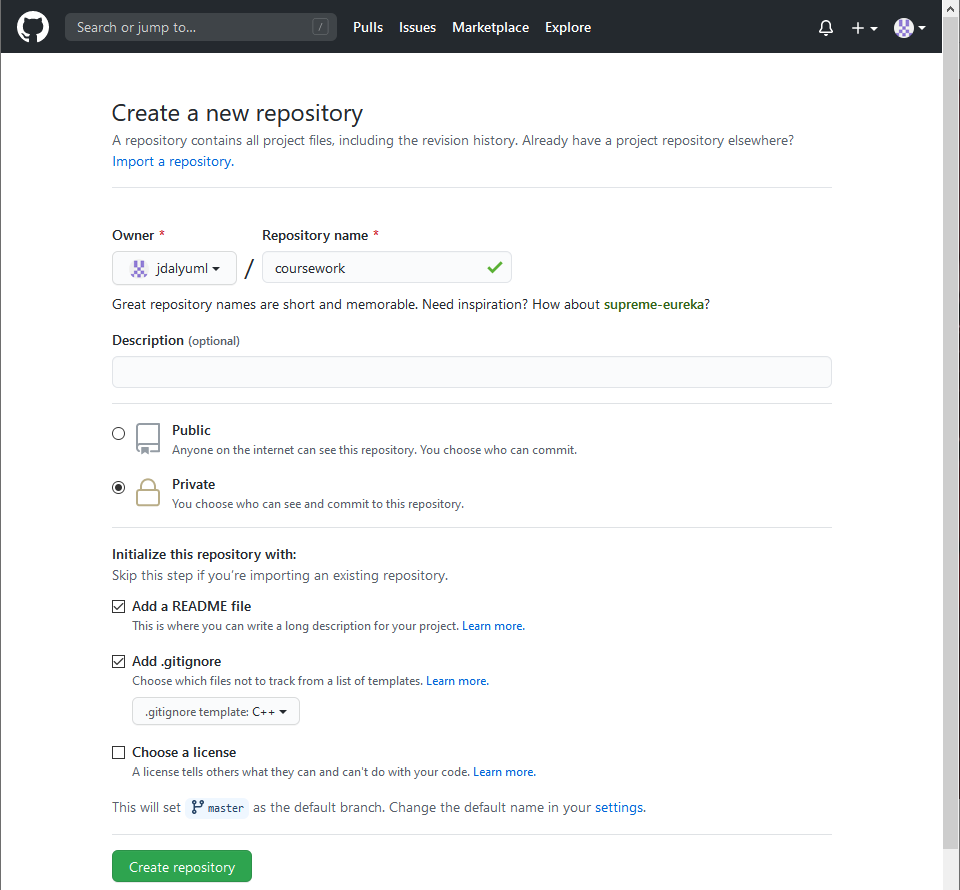
\includegraphics[width=0.7\columnwidth]{newrepo}

Once you have created your repository, go to the Settings tab, then select Manage Access and invite the instructor (jdalyuml) as a collaborator.
This will allow us access to the repository even though it is a private repository.
Once this assignment has been graded you can remove them as a collaborator.

Now, we will clone the repository to your machine and put some starter material into the repository.
Open a terminal (using the Git Bash terminal on Windows) and navigate to the directory where you want to copy the repository.
You can clone the repository using the command \code{git clone <repo url>} where \code{<repo url>} can be found on the Code tab of your GitHub repository by selecting the \textcolor{green}{green} download code button.
Once you have downloaded the repository, create a directory for whichever CS courses you are currently taking (e.g. Computing I) or that you expect to take next if you are not currently taking one.
Optionally, you can create subdirectories for your current assignments.
This will give you a place to keep the work for your other classes.

If you use \code {git status} you can see that you have added some files or at least a directory.
Use \code{git add <filename>} to add your new class directory and any other wanted files to the staging area.
Once you have selected all of the files you want, you can commit the changes by using \code{git commit -m <some message>}.
This commits the changes to your local repository, but doesn't update GitHub.
Use \code{git push} to send your changes back to GitHub.

Once you've verified that your repository has been updated on GitHub, submit a link to your repository on Blackboard.
\end{document}